% Problem and Scope
Autonomous robotic systems are required to operate under limited resources (e.g., task allocation, computational budget, and battery capacity), making efficient resource utilization a critical requirement for real-world deployment~\cite{gerkey2004formal, afrin2021resource, dai2022multi, hai2025replanning, liao2025sa}.
This challenge is particularly critical in dynamic environments, where agents must make rapid decisions in response to fast-changing situations~\cite{hai2025replanning, liao2025sa}.
In this work, we consider a tactical decision-making problem by viewing resource usage as part of robotic actions, where each action incurs a finite resource cost.
Effective control over such resource-usage actions must be coordinated with the generation of subsequent maneuvers, as each decision determines not only how resources are consumed but also how their effects can be maximized through follow-up actions.

% Key challenges & hybrid action RL (narrow scope)
Addressing tactical decision-making under resource constraints requires explicit modeling of hybrid action spaces that combine resource usage with maneuver control.
These hybrid structures naturally arise in practice: discrete actions govern resource usage (e.g., weapon release in Fig.~\ref{fig:main-figure}), while continuous actions guide low-level behaviors such as motion control~\cite{hausknecht2015deep}.
Although reinforcement learning (RL) has been widely applied in these domains~\cite{hausknecht2015deep, masson2016reinforcement, xiong2018parametrized, fan2019hybrid, li2021hyar}, existing approaches often overlook two aspects that are particularly critical in tactical decision-making: \textit{causal dependency} and \textit{multi-modality}.
Causal reasoning is necessary to predict how resource usage constrains future maneuvers.
Multi-modality is essential in dynamic environments such as air combat or mobile robot navigation, where the same discrete decision may lead to multiple valid follow-up maneuvers depending on the evolving situation (Fig.~\ref{fig:main-figure}).
Conventional RL approaches neglect these properties, thereby converging to a single dominant policy and limiting tactical flexibility~\cite{wu2025discrete}.

\begin{figure}[t!]
\centering
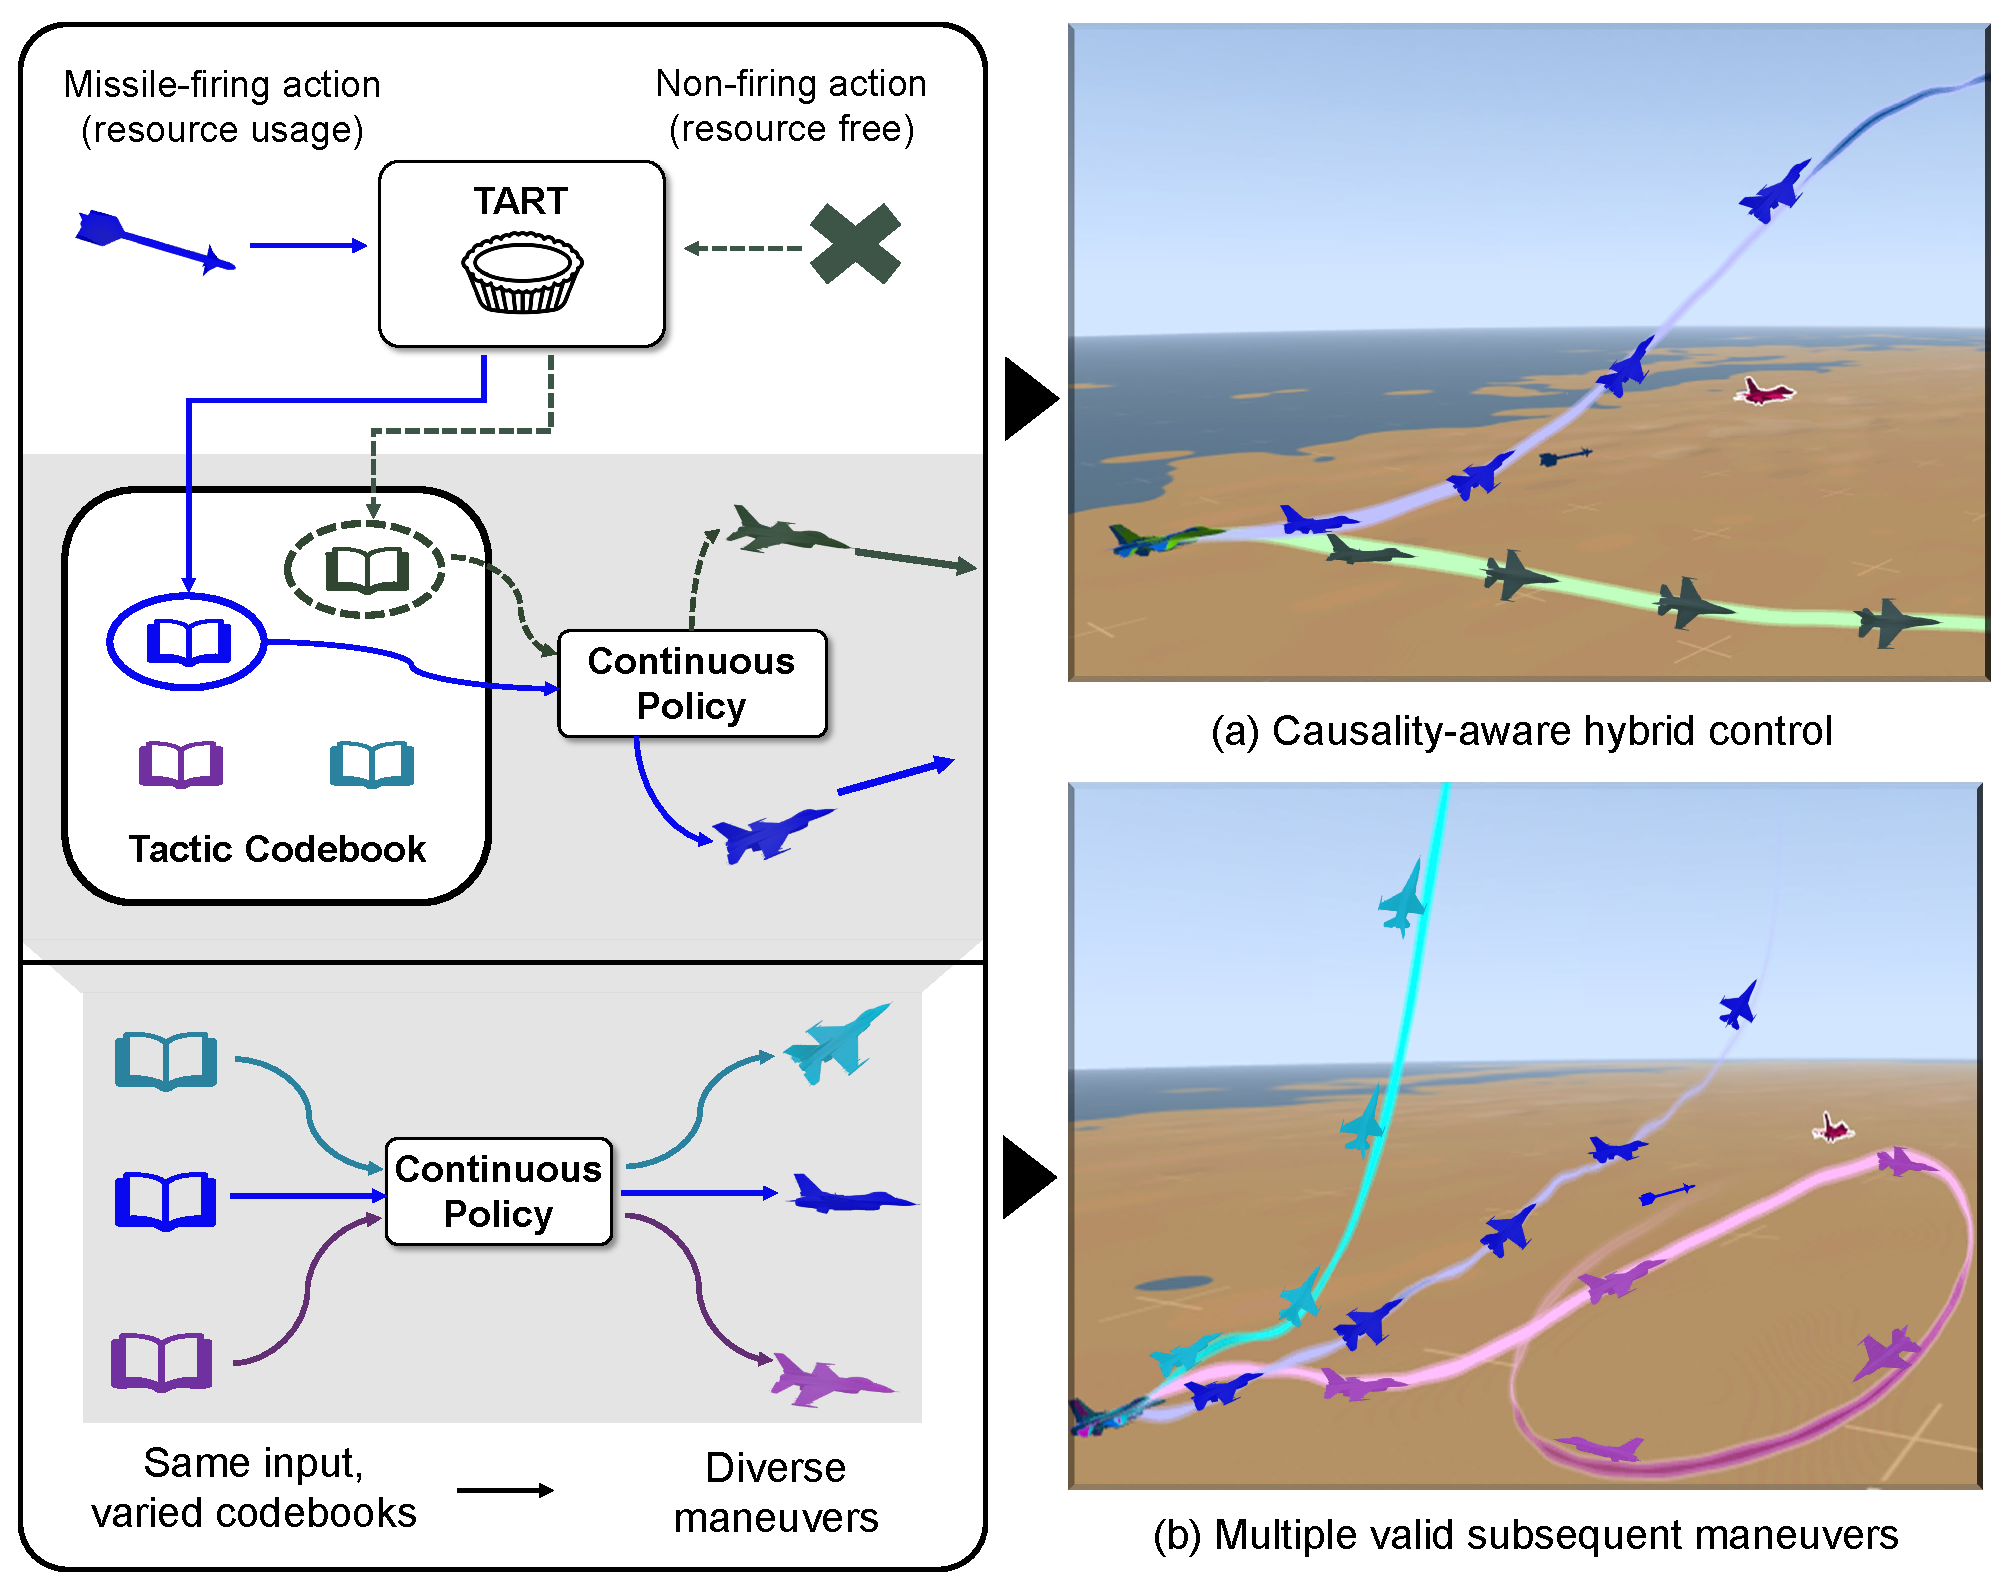
\includegraphics[width=\columnwidth]{Figures/fig_1.pdf}
\caption{Snapshots of tactical decision-making in an air combat scenario. (a) A discrete action (e.g., weapon release) both constrains the set of feasible follow-up maneuvers (\textit{causal dependency}) and (b) gives rise to multiple valid maneuver modes (\textit{multi-modality}). TART is designed to capture these temporal dependencies and multi-modal outcomes, conditioning the policy to select context-appropriate maneuvers.
\vspace{-20pt}
}
\label{fig:main-figure}
\end{figure}

% Structural Challenge : Need for Representation learning
These challenges highlight the need for temporal representation learning of robotic actions that can jointly capture resource usage, causal effects, and maneuver diversity.
This necessity arises from the hierarchical structure of decision-making, where discrete resource-allocation decisions are temporally coupled with continuous maneuver controls.
Representation learning provides a means to abstract these interactions into structured latent embeddings, enabling policies to reason over temporal dependencies~\cite{ze2023visual, biza2025robot, bu2025univla} while preserving the diversity of valid maneuver outcomes~\cite{mehta2022learning ,luo2023action, zhu2023imitation}.
Such compact representations are largely absent in prior RL approaches to scalable and resource-aware robotic decision-making, underscoring the importance of temporally grounded action representations.

% Method
In this paper, we propose \textbf{T}emporal \textbf{A}ction \textbf{R}epresentation learning for \textbf{T}actical resource control and subsequent maneuver generation (TART), a framework for learning temporally grounded representations for hybrid action policies.
The core idea is to model the conditional distribution of continuous maneuvers given recent state history with the current discrete resource usage decision.
We realize this by maximizing a mutual information objective via a trajectory-level contrastive loss that aligns matched context--future pairs and separates mismatched pairs~\cite{oord2018representation}.
The resulting context embeddings are vector-quantized into a compact, interpretable codebook of tactical modes~\cite{van2017neural}.
These codes condition a factorized hybrid policy where discrete actions feed into the representation to select a tactical mode, and the resulting mode guides a continuous actor to produce a multi-modal maneuver distribution.
Our representation learning framework integrates into the standard on-policy RL loop, being updated jointly with policy optimization~\cite{schulman2017proximal}.
By grounding action representations temporally and structuring them into discrete tactical modes, TART preserves maneuver multi-modality while enforcing resource-aware consistency under hybrid action spaces.

We evaluate TART in two domains that combine resource constraints with hybrid action spaces.
The first is a maze navigation task where agents have a limited budget of discrete boost and wall penetration actions that enhance mobility alongside continuous movement.
The second is a high-fidelity air-to-air combat simulator where an F-16 agent coordinates continuous flight control with discrete weapon and defense system deployment.
Across both domains, TART outperforms standard hybrid-action baselines and generates behaviors that capture causal dependencies and support multi-modal tactical decisions.
These results underscore the importance of structured action representations that encode temporal dependencies, enabling resource-aware robotic decision-making.

The contributions of our work are as follows:

\begin{itemize}
    \item We introduce TART, a temporal action representation learning framework that unifies resource control and maneuver generation to address tactical decision-making under resource limits in hybrid action spaces.
    \item We propose a mutual information-based objective with trajectory-level contrastive learning and a vector-quantized codebook, resulting in representations that capture causal dependencies and support multi-modal, temporally coherent behaviors.
    \item We conduct extensive experiments in both maze navigation and air-to-air combat environments, demonstrating (i) superior performance over hybrid-action baselines, (ii) improved modeling of maneuver multi-modality and temporal coherence in hybrid action sequences.
\end{itemize}